\section{Quotient Groups and Homomorphisms}

\subsection{Definitions and Examples}

Let $G$ and $H$ be groups.

\begin{exercise}[3.1.1]
    Let $\phi : G \to H$ be a homomorphism and let $E$ be a subgroup of $H$.
	Prove that $\phi\inv(E) \leq G$.
	If $E \nsub H$ prove that $\phi\inv(E) \nsub G$.
	Deduce that $\ker(\phi) \nsub G$.
\end{exercise}

\begin{sol}
    Observe that $1_G \in \phi\inv(E)$ since $\phi(1_G) = 1_H \in E$.
	Let $x, y \in \phi\inv(E)$ so that $\phi(x), \phi(y) \in E$.
	Since $E \leq H$, then $\phi(xy\inv) = \phi(x)\phi(y)\inv \in E$, hence $xy\inv \in \phi\inv(E)$.
	Therefore, $\phi\inv(E) \leq G$.

    Suppose $E \nsub H$.
	Then $heh\inv \in E$ for all $h \in H$ and $e \in H$.
	Let $x \in \phi\inv(E)$ and $g \in G$.
	Then
    \[
    	\phi(gxg\inv) = \phi(g)\phi(x)\phi(g)\inv \in E,
    \]
    so that $gxg\inv \in \phi\inv(E)$.
	Therefore, $\phi\inv(E) \nsub G$.
	Then $\ker \phi = \phi\inv(1_H) \nsub G$ since $\set{1_H} \nsub H$.
\end{sol}

\begin{exercise}[3.1.2]
    Let $\phi : G \to H$ be a homomorphism of groups with kernel $K$ and let $a,b \in \phi(G)$.
	Let $X \in G/K$ be the fiber above $a$ and let $Y$ be the fiber above $b$, i.e., $X = \phi\inv (a)$, $Y = \phi\inv (b)$.
	Fix an element $u \in X$ (so $\phi(u)=a$).
	Prove that if $XY = Z$ in the quotient group $G/K$ and $w$ is any member of $Z$, then there is some $v \in Y$ such that $uv = w$.
    
    \hint{Show $u\inv w \in Y$.}
\end{exercise}

\begin{sol}
    Let $w \in Z$, and define $v = u\inv w$.
	Then
    \[
    	\phi(v) = \phi(u\inv w) = \phi(u)\inv \phi(w) = a\inv (ab) = b
    \]
    so that $v \in Y$ and $uv = w$.
\end{sol}

\begin{exercise}[3.1.3]
    Let $A$ be an Abelian group and let $B$ be a subgroup of $A$.
	Prove that $A/B$ is Abelian.
	Give an example of a non-Abelian group $G$ containing a proper normal subgroup $N$ such that $G/N$ is Abelian.
\end{exercise}

\begin{sol}
    Let $aB, a'B \in A/B$.
	Then
    \[
    	(aB)(a'B) = (aa')B = (a'a)B = (a'B)(aB)
    \]
    so that $A/B$ is Abelian.

    To obtain Abelian quotient groups, consider non-Abelian groups and their centers.
	Put $G = D_8$ and $N = Z(D_8) = \gen{r^2}$.
	Then $G/N \cong V_4$ is Abelian.
\end{sol}

\begin{exercise}[3.1.4]
    Prove that in the quotient group $G/N$, $(gN)^{\alpha} = g^{\alpha}N$ for all $\alpha \in \z$.
\end{exercise}

\begin{sol}
    Inducting on $\alpha$, the base case $\alpha = 0$ is clear since $(gN)^0 = N = g^0N$.
	Suppose the statement holds for some $\alpha \in \z$.
	Then
    \[
    	(gN)^{\alpha + 1} = (gN)^{\alpha}(gN) = g^{\alpha}N gN = g^{\alpha + 1}N.
    \]
    Hence, the statement holds for all $\alpha \in \zp \cup \set 0$.
	The case of $\alpha = -1$ is handled by Proposition 3.5.
	For all negative $\alpha$, utilize $\alpha = -1$ and the positive case to obtain the result.
\end{sol}

\begin{exercise}[3.1.5]
    Use the preceding exercise to prove that the order of the element $gN$ in $G/N$ is $n$, where $n$ is the smallest positive integer such that $g^n \in N$ (and $gN$ has infinite order if no such positive integer exists).
	Give an example to show that the order of $gN$ in $G/N$ may be strictly smaller than the order of $g$ in $G$.
\end{exercise}

\begin{sol}
    Let $gN \in G/N$.
	If there exists some $n \in \zp$ such that $g^n \in N$, then \exref{3.1.4} shows that $(gN)^n = g^nN = N$, so that the order of $gN$ is at most $n$.
	If there exists some $m < n$ such that $(gN)^m = N$, then \exref{3.1.4} shows that $g^m \in N$, contradicting the minimality of $n$.
	Hence, the order of $gN$ is exactly $n$.
	If no such positive integer exists, then $(gN)^m \neq N$ for all $m \in \zp$.
	If $|gN|$ were finite, then there would exist some $m \in \zp$ such that $(gN)^m = N$, contradicting the assumption.
	Hence, $|gN|$ is infinite.

    Put $G = Z_4 = \gen x$ and $N = \gen{x^2}$.
	Then $|x| = 4$, but $|xN| = 2$ since $(xN)^2 = x^2N = N$.
\end{sol}

\begin{exercise}[3.1.6]
    Define $\phi : \r^{\times} \to \set{\pm 1}$ by letting $\phi(x)$ be $x$ divided by the absolute value of $x$.
	Describe the fibers of $\phi$ and prove that $\phi$ is a homomorphism.
\end{exercise}

\begin{sol}
    $\phi\inv(+1)$ consists of positive reals and $\phi\inv(-1)$ negative reals.
	Let $x, y \in \r\unt$.
	Then
    \[
    	\phi(xy) = \frac{xy}{\abs{xy}} = \frac{x}{\abs x} \cdot \frac{y}{\abs y} = \phi(x)\phi(y) \qh
    \]
\end{sol}

\begin{exercise}[3.1.7]
    Define $\pi : \r^2 \to \r$ by $\pi((x,y)) = x + y$.
	Prove that $\pi$ is a surjective homomorphism and describe the kernel and fibers of $\pi$ geometrically.
\end{exercise}

\begin{sol}
    Let $(x_1, y_1), (x_2, y_2) \in \r^2$.
	Then
    \[
    	\pi((x_1, y_1) + (x_2, y_2)) = (x_1 + x_2) + (y_1 + y_2) = (x_1 + y_1) + (x_2 + y_2) = \pi((x_1, y_1)) + \pi((x_2, y_2)),
    \]
    hence $\pi$ is a homomorphism.
	Moreover, $\pi$ is surjective since $\pi((a, 0)) = a$ for all $a \in \r$.
	We have $\ker\pi$ as the line $y = -x$, and $\pi\inv(a)$ as $y = a - x$, which is $\ker\pi$ translated up by $a$.
\end{sol}

\begin{exercise}[3.1.8]
    Let $\phi : \r^{\times} \to \r^{\times}$ be the map sending $x$ to the absolute value of $x$.
	Prove that $\phi$ is a homomorphism and find the image of $\phi$.
	Describe the kernel and the fibers of $\phi$.
\end{exercise}

\begin{sol}
    Let $x, y \in \r\unt$.
	Then
    \[
    	\phi(xy) = \abs{xy} = \abs x \abs y = \phi(x)\phi(y)
    \]
    so that $\phi$ is a homomorphism.
	Note that $\abs x > 0$ for any $x \in \r\unt$, so $\im(\phi) = \r^+$. $\ker(\phi) = \set{-1, 1}$, and the fiber of $\phi$ over some $a \in \r^+$ is simply $\set{-a, a}$.
\end{sol}

\begin{exercise}[3.1.9]
    Define $\phi : \c^{\times} \to \r^{\times}$ by $\phi(a+bi) = a^2 + b^2$.
	Prove that $\phi$ is a homomorphism and find the image of $\phi$.
	Describe the kernel and the fibers of $\phi$ geometrically (as subsets of the plane).
\end{exercise}

\begin{sol}
    Let $a + bi, c + di \in \c\unt$.
	Then
    \begin{align*}
        \phi((a + bi)(c + di)) & = \phi((ac - bd) + (ad + bc)i) \\
        & = (ac - bd)^2 + (ad + bc)^2 \\
        & = a^2c^2 - 2abcd + b^2d^2 + a^2d^2 + 2abcd + b^2c^2 \\
        & = (a^2 + b^2)(c^2 + d^2) \\
        & = \phi(a + bi)\phi(c + di)
    \end{align*}
    so that $\phi$ is a homomorphism.
	Observe that $a^2 + b^2 > 0$ for any $a + bi \in \c\unt$, so that $\im(\phi) = \r^+$. $\ker\phi$ is the unit circle in the complex plane, and the fiber of $\phi$ over some $r \in \r^+$ is the circle of radius $\sqrt r$ centered at the origin.
\end{sol}

\begin{exercise}[3.1.10]
    Let $\phi : \intmod[8] \to \intmod[4]$ by $\phi(\bar  a) = \bar  a$.
	Show that this is a well-defined, surjective homomorphism and describe its fibers and kernel explicitly (showing that $\phi$ is well-defined involves the fact that $\bar  a$ has a different meaning in the domain and range of $\phi$).
\end{exercise}

\begin{sol}
    To show that $\phi$ is well-defined, suppose $\bar a = \bar b$ in $\intmod[8]$.
	Then $8 \mid (a - b)$, so that $a - b = 8k$ for some $k \in \z$.
	Then $a - b = 4(2k)$, so that $4 \mid (a - b)$ and $\bar a = \bar b$ in $\intmod[4]$.
	Hence, $\phi$ is well-defined.
	Moreover, for any $\bar a, \bar b \in \intmod[8]$, then
    \[
    	\phi(\bar a + \bar b) = \phi(\overline{a + b}) = \overline{a + b} = \bar a + \bar b = \phi(\bar a) + \phi(\bar b)
    \]
    so that $\phi$ is a homomorphism.
	Note that for any $\bar c \in \intmod[4]$, then $\phi(\bar c) = \bar c$, so $\phi$ is surjective.
	The fibers of $\phi$:
    \begin{align*}
        \phi\inv(\bar 0) & = \set{\bar 0, \bar 4} \\
        \phi\inv(\bar 1) & = \set{\bar 1, \bar 5} \\
        \phi\inv(\bar 2) & = \set{\bar 2, \bar 6} \\
        \phi\inv(\bar 3) & = \set{\bar 3, \bar 7}
    \end{align*}
    with $\ker\phi = \phi\inv(\bar 0) = \set{\bar 0, \bar 4}$.
\end{sol}

\begin{exercise}[3.1.11]
    Let $F$ be a field and let
    \[
    	G = \set*{\left.
        \begin{pmatrix}
            a & b \\
            0 & c 
        \end{pmatrix}~\right|~a, b, c \in F, ac \neq 0} \leq \gl_2(F)
	\]
    \begin{subexercises}
        \item Prove that the map
        \[
        	\phi : 
            \begin{pmatrix}
                a & b \\
                0 & c
            \end{pmatrix} \mapsto a
	    \]
        is a surjective homomorphism from $G$ onto $F\unt$ (recall that $F\unt$ is the multiplicative group of nonzero elements in $F$).
	    Describe the fibers and kernel of $\phi$.
        \item Prove that the map
        \[
        	\psi : 
            \begin{pmatrix}
                a & b \\
                0 & c
            \end{pmatrix} \mapsto (a, c)
        \]
        is a surjective homomorphism from $G$ onto $F\unt \times F\unt$.
	    Describe the fibers and kernel of $\psi$. 
        \item Let
        \[
        	H = \set*{\left .
            \begin{pmatrix}
                1 & b \\
                0 & 1
            \end{pmatrix} ~\right\vert~b \in F}
        \]
        Prove that $H$ is isomorphic to the additive group $F$.
    \end{subexercises}
\end{exercise}

\begin{solenum}
    \item Observe that
    \[
    	\phi\left(
        \begin{pmatrix}
            a & 1 \\
            0 & 1
        \end{pmatrix}\right) = a
	\]
    so that $\phi$ is surjective.
	Moreover, for any $a, b, c, d, e, f \in F$ with $ac \neq 0$ and $df \neq 0$, we have
    \[
    	\phi\left(
        \begin{pmatrix}
            a & b \\
            0 & c
        \end{pmatrix}
        \begin{pmatrix}
            d & e \\
            0 & f
        \end{pmatrix}\right) = 
        \phi\left(
        \begin{pmatrix}
            ad & ae + bf \\
            0 & cf
        \end{pmatrix}\right) = ad = 
        \phi\left(
        \begin{pmatrix}
            a & b \\
            0 & c
        \end{pmatrix}\right)
        \phi\left(
        \begin{pmatrix}
            d & e \\
            0 & f
        \end{pmatrix}\right)
	\]
    and $\phi$ is then a homomorphism.
	The fiber of $a \in F\unt$ over $\phi$ is
    \[
    	\phi\inv(a) = 
        \set*{\left.
        \begin{pmatrix}
            a & s \\
            0 & t
        \end{pmatrix}~\right|~s, t \in F, t \neq 0}
	\]
    with $\ker\phi = \phi\inv(1)$.
    \item To show that $\psi$ is surjective is similar as the previous exercise.
	The fiber of any $(a, c) \in F\unt \times F\unt$ is
    \[
    	\psi\inv((a, c)) = 
        \set*{\left.
        \begin{pmatrix}
            a & s \\
            0 & c
        \end{pmatrix}~\right|~s \in F}
	\]
    with $\ker\psi = \psi\inv((1, 1))$.
    \item Define the mapping $\pi_1 : H \to F$ given by
    \[
    	\pi_1\left(
        \begin{pmatrix}
            1 & b \\
            0 & 1
        \end{pmatrix}\right) = b
	\]
    Define another map $\pi_2 : F \to H$ given by
    \[
    	\pi_2(b) = 
        \begin{pmatrix}
            1 & b \\
            0 & 1
        \end{pmatrix}
	\]
    It is clear that $\pi_2$ is a two-sided inverse of $\pi_1$.
	For any $b, c \in F$, we have
    \[
    	\pi_1\left(
        \begin{pmatrix}
            1 & b \\
            0 & 1
        \end{pmatrix}
        \begin{pmatrix}
            1 & c \\
            0 & 1
        \end{pmatrix}\right) = 
        \pi_1\left(
        \begin{pmatrix}
            1 & b + c \\
            0 & 1
        \end{pmatrix}\right) = b + c = 
        \pi_1\left(
        \begin{pmatrix}
            1 & b \\
            0 & 1
        \end{pmatrix}\right) + 
        \pi_1\left(
        \begin{pmatrix}
            1 & c \\
            0 & 1
        \end{pmatrix}\right)
	\]
    so that $\pi_1$ is a homomorphism.
	Then $\pi_1$ is an isomorphism, and $H \cong F$.
\end{solenum}

\begin{exercise}[3.1.12]
    Let $G$ be the additive group of real numbers, let $H$ be the multiplicative group of complex numbers of absolute value $1$ (the unit circle $S^1$ in the complex plane) and let $\phi : G \to H$ be the homomorphism $\phi : r \mapsto e^{2\pi i r}$.
	Draw the points on a real line which lie in the kernel of $\phi$.
	Describe similarly the elements in the fibers of $\phi$ above the points $-1$, $i$, and $e^{4\pi i/3}$ of $H$.
\end{exercise}

\begin{sol}
    Since $e^{2\pi ir} = 1$ if and only if $r$ is an integer, then $\ker(\phi) = \z$.
	On a number line, this is shown as
    \begin{center}
        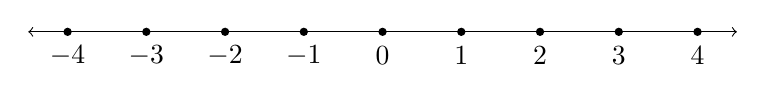
\begin{tikzpicture}
            \draw[<->] (-4.5, 0) -- (4.5, 0);

            \foreach \x in {-4, -3, -2, -1, 0, 1, 2, 3, 4}
                \fill (\x, 0) circle (1.5pt);

            \foreach \x in {-4, -3, -2, -1, 0, 1, 2, 3, 4}
                \node at (\x, -0.3) {$\x$};
        \end{tikzpicture}
    \end{center}
    Moreover, note that $-1 = e^{-2\pi i/2}$ and $i = e^{2\pi i/4}$.
	Then the fibers of these elements are just the integral differences of $1/2, 1/4$, and $2/3$ respectively, since $4\pi i/3 = 2/3(2\pi i)$:
    \begin{align*}
        \phi\inv(-1) & = \frac 12 + \z = \set*{\left.\frac 12 + n~\right|~n \in \z} \\
        \phi\inv(i) & = \frac 14 + \z = \set*{\left.\frac 14 + n~\right|~n \in \z} \\
        \phi\inv(e^{4\pi i/3}) & = \frac 23 + \z = \set*{\left.\frac 23 + n~\right|~n \in \z} \qh
    \end{align*}
\end{sol}

\begin{exercise}[3.1.13]
    Repeat the preceding exercise with the map $\phi$ replaced by the map $\phi : r \mapsto e^{4\pi i r}$.
\end{exercise}

\begin{sol}
    The kernel of $\phi$ is $\frac12\z$, or
    \begin{center}
        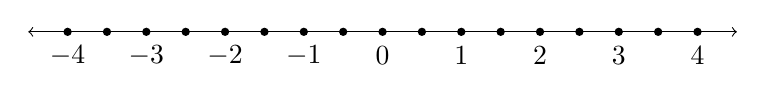
\begin{tikzpicture}
            \draw[<->] (-4.5, 0) -- (4.5, 0);

            \foreach \x in {-4, -3.5, -3, -2.5, -2, -1.5, -1, -0.5, 0, 0.5, 1, 1.5, 2, 2.5, 3, 3.5, 4}
                \fill (\x, 0) circle (1.5pt);

            \foreach \x in {-4, -3, -2, -1, 0, 1, 2, 3, 4}
                \node at (\x, -0.3) {$\x$};
        \end{tikzpicture}
    \end{center}
    Moreover, the fibers are just all halved, so
    \begin{align*}
        \phi\inv(-1) & = \frac14 + \frac12 \z = \set*{\left.\frac14 + \frac n2~\right|~n \in \z} \\
        \phi\inv(-i) & = \frac18 + \frac12 \z = \set*{\left.\frac18 + \frac n2~\right|~n \in \z} \\
        \phi\inv(e^{4\pi i/3}) & = \frac13 + \frac12 \z = \set*{\left.\frac13 + \frac n2~\right|~n \in \z} \qh
    \end{align*}
\end{sol}

\begin{spex}[3.1.14]
    Consider the additive quotient group $\q/\z$.
    \begin{subexercises}
        \item Show that every coset of $\z$ in $\q$ contains exactly one representative $q \in \q$ in the range $0 \le q < 1$.
        \item Show that every element of $\q/\z$ has finite order but that there are elements of arbitrarily large order.
        \item Show that $\q/\z$ is the torsion subgroup of $\r/\z$ (cf. \exref{2.1.6}).
        \item Prove that $\q/\z$ is isomorphic to the multiplicative group of roots of unity in $\c^\times$.
    \end{subexercises}
\end{spex}

\begin{solenum}
    \item Suppose $a/b \in \q$ with $(a, b) = 1$.
	By the Division Algorithm, there exist unique integers $q, r$ such that $a = bq + r$ for $0 \leq r < b$, or equivalently, $a/b = q + r/b$.
	Then $a/b + \z = r/b + \z$.
	If there exists some other representative $s/t$ in $0 \leq s/t < 1$ such that $a/b + \z = s/t + \z$, then $r/b + \z = s/t + \z$, or that $r/b - s/t \in \z$.
	Then there exists some integer $k$ such that $rt - sb = kbt$.
	Since $0 \leq r < b$ and $0 \leq s < t$, then $0 \leq rt < bt$ and $0 \leq sb < bt$.
	Combining these two inequalities, we get $-bt < rt - sb < bt$, so that $-1 < k < 1$.
	Since $k$ is an integer, then $k = 0$, and $rt - sb = 0$, or $r/b = s/t$.
	Hence, the representative in $0 \leq q < 1$ is unique.
    \item Let $a/b \in \q$.
	Then $b(a/b + \z) = ab + \z = \z$, so that $a/b + \z$ has finite order.
	Moreover, $1/k + \z \in \q/\z$ has order $k$, and since $k$ can be made arbitrarily large, then there are elements of arbitrarily large order.
    \item By the previous exercise, $\q/\z \subseteq \tor(\r/\z)$.
	Let $x + \z \in \tor(\r/\z)$.
	Then $|x + \z|$ is finite, so there exists some $n \in \z$ such that $n(x + \z) = nx + \z = \z$.
	Then $nx \in \z$, so that $x = m/n$ for some $m \in \z$.
	Hence, $x + \z \in \q/\z$, and $\tor(\r/\z) \subseteq \q/\z$.
	Therefore, $\tor(\r/\z) = \q/\z$.
    \item By \exref{3.1.12}, we have $\r/\z \cong S^1$.
	By definition, $\tor(S^1)$ consists of $z \in \c\unt$ such that $z^n = 1$ for some $n \in \zp$.
	This is precisely the set of roots of unity.
	Since $\tor(\r/\z) = \q/\z$, then $\q/\z$ is isomorphic to the set of roots of unity.
\end{solenum}

\begin{exercise}[3.1.15]
    Prove that a quotient of a divisible Abelian group by any proper subgroup is also divisible.
	Deduce that $\q/\z$ is divisible (cf. \exref{2.4.19}).
\end{exercise}

\begin{sol}
    Since $A$ is Abelian, any proper subgroup $B$ of $A$ is normal.
	To that end, let $aB \in A/B$, and let $n \in \zp$.
	Since $A$ is divisible, there exists some $x \in A$ such that $x^n = a$.
	Then
    \[
    	(xB)^n = x^n B = aB
    \]
    so that $A/B$ is divisible.
	Observe that $\q$ is divisible, since for any $q \in \q$ and $n \in \zp$, there exists $p \in \q$ such that $np = q$, namely $p = q/n$.
	Moreover, $\z$ is a proper subgroup of $\q$, so by the first part, $\q/\z$ is divisible.
\end{sol}

\begin{spex}[3.1.16]
    Let $G$ be a group, let $N$ be a normal subgroup of $G$, and let $\bar{G} = G/N$.
	Prove that if $G = \langle x, y \rangle$ then $\bar{G} = \langle \bar{x}, \bar{y} \rangle$.
	Prove more generally that if $G = \langle S \rangle$ for any subset $S$ of $G$, then $\bar{G} = \langle \bar{S} \rangle$.
\end{spex}

\begin{sol}
    We prove the general case.
	Since $G = \gen S$, then for any $g \in G$, we have
    \[
    	g = s_1^{\alpha_1} s_2^{\alpha_2} \cdots s_k^{\alpha_k}, \quad s_i \in S, \alpha_i \in \z
    \]
    Observe that $\bar S = \set{\bar s \mid s \in S}$.
	Then for any $\bar g \in \bar G$, we have
    \[
    	\bar g = \bar{s_1^{\alpha_1} s_2^{\alpha_2} \cdots s_k^{\alpha_k}} = \bar s_1^{\alpha_1} \bar s_2^{\alpha_2} \cdots \bar s_k^{\alpha_k}
    \]
    so that $\bar g \in \gen{\bar S}$.
	Hence, $\bar G \subseteq \gen{\bar S}$.
	Since $\bar s \in \bar G$ for any $s \in S$, then $\gen{\bar S} \subseteq \bar G$.
	Therefore, $\bar G = \gen{\bar S}$.

    The case of $G = \gen{x, y}$ is a special case where $S = \set{x, y}$.
\end{sol}

\begin{exercise}[3.1.17]
    Let $G$ be the dihedral group of order $16$ (whose lattice appears in Section 2.5): $G = \langle r,s \mid r^8 = s^2 = 1,\ rs = sr\inv  \rangle$, and let $\bar{G} = G/\langle r^4 \rangle$ be the quotient of $G$ by the subgroup generated by $r^4$ (this subgroup is the center of $G$, hence is normal).
    \begin{subexercises}
        \item Show that the order of $\bar{G}$ is $8$.
        \item Exhibit each element of $\bar{G}$ in the form $\bar{s}^a \bar{r}^b$, for some integers $a$ and $b$.
        \item Find the order of each of the elements of $\bar{G}$ exhibited in (b).
        \item Write each of the following elements of $\bar{G}$ in the form $\bar{s}^a \bar{r}^b$, for some integers $a$ and $b$ as in (b): $\bar{rs}$, $\bar{sr^{-2}s}$, $\bar{s\inv r\inv sr}$.
        \item Prove that $\bar{H} = \langle \bar{s}, \bar{r}^2 \rangle$ is a normal subgroup of $\bar{G}$ and $\bar{H}$ is isomorphic to the Klein $4$-group.
	    Describe the isomorphism type of the complete preimage of $\bar{H}$ in $G$.
        \item Find the center of $\bar G$ and describe the isomorphism type of $\bar G/Z(\bar G)$.
    \end{subexercises}
\end{exercise}

\begin{solenum}
    \item Since $\gen{r^4} = \set{1, r^4}$, each coset in $\bar G$ has 2 elements and partitions $G$ into 8 sets.
	Hence, $\abs{\bar G} = 8$.
    \item The elements of $\bar G$ are
    \begin{align*}
        \bar 1 & = \set{1, r^4}, & \bar{s} & = \set{s, sr^4} \\
        \bar r & = \set{r, r^5}, & \bar{sr} & = \set{sr, sr^5} \\
        \bar r^2 & = \set{r^2, r^6}, & \bar{sr^2} & = \set{sr^2, sr^6} \\
        \bar r^3 & = \set{r^3, r^7}, & \bar{sr^3} & = \set{sr^3, sr^7}
    \end{align*}
    \item The orders of the elements of $\bar G$ are
    \[
        \begin{array}{c|c|c|c|c|c|c|c|c}
            \bar x & \bar 1 & \bar r & \bar r^2 & \bar r^3 & \bar s & \bar{sr} & \bar{sr^2} & \bar{sr^3} \\
            \hline
            \abs x & 1 & 4 & 2 & 4 & 2 & 2 & 2 & 2
        \end{array}
    \]
    \item $\bar{rs} = \bar{sr^3}, \bar{sr^{-2}s} = \bar r^2, \bar{s\inv r\inv sr} = \bar r^2$.
    \item We first note that $\bar H = \set{1, \bar r^2, \bar s, \bar{sr^2}}$.
	To show that $\bar H \nsub \bar G$, we simplify the process by noting that elements of $\bar G$ are of the form $\bar r^k$ or $\bar{sr^k}$.
	If an element is of the former, we have
    \begin{align*}
        \bar{r^kr^2r^{-k}} = \bar r^2 \in \bar H \\
        \bar{r^ksr^{-k}} = \bar{s(r^2)^{-k}} \in \bar H
    \end{align*}
    If it is of the latter, then
    \begin{align*}
        \bar{(sr^k)r^2(r^{-k}s)} = \bar{r^{-2}} \in H \\
        \bar{(sr^k)s(r^{-k}s)} = \bar{s(r^2)^k} \in H
    \end{align*}
    where $\bar{sr^k}\inv = \bar{r^{-k}s}$.
	The above calculations show that for every $\bar g \in \bar G$, then $\bar{gr^2g\inv}, \bar{gsg\inv} \in H$ so that $\bar{gHg\inv} = \bar H$, hence $\bar H \nsub \bar G$.
	Moreover, it is easy to see that every element of $\bar H$ is of order 2 so that $\bar H \cong V_4$.

    Let $\pi : G \to \bar G$ be the natural projection of $G$ onto $\bar G$.
	Then $\pi\inv(\bar H)$ is the complete preimage of $\bar H$, or the set of elements that map to a coset in $\bar H$.
	Using part (b), we see that
    \[
    	\pi\inv(\bar H) = \set{1, r^2, r^4, r^6, s, sr^2, sr^4, sr^6}
    \]
    Note that $|\pi\inv(\bar H)| = 8$, and the elements of $\bar H$ satisfy the relations $(r^2)^4 = s^2 = 1$.
	Then the mapping $\phi : D_8 \to \pi\inv(\bar H)$ given by $\phi(r) = r^2$ and $\phi(s) = s$ extends to a homomorphism that is clearly surjective.
	Then $\phi$ is an isomorphism, and $\pi\inv(\bar H) \cong D_8$.
    \item From the previous exercise, we have that $\bar G = \gen{\bar r, \bar s}$.
	Since $\bar r^2$ commutes with both $\bar r$ and $\bar s$, then $\bar r^2 \in Z(\bar G)$.
	However, $\bar{rs} \neq \bar{sr}$ and $\bar{r^3s} \neq \bar{sr^3}$.
	Additionally, none of $\bar{sr}, \bar{sr^2}$, nor $\bar{sr^3}$ commute with $\bar r$ so that $Z(\bar G) = \set{\bar 1, \bar r^2}$.
	The elements of $\widehat G = \bar G/Z(\bar G)$ are as follows:
    \begin{align*}
        \wh 1 & = \set{\bar 1, \bar r^2} & \wh s & = \set{\bar s, \bar{sr^2}} \\
        \wh r & = \set{\bar r, \bar r^3} & \widehat{sr} & = \set{\bar{sr}, \bar{sr^3}}
    \end{align*}
    One can see that each non-identity element of $\widehat G$ has order 2 so that $\widehat G \cong V_4$.
\end{solenum}

\begin{exercise}[3.1.18]
    Let $G$ be the quasidihedral group of order $16$ (whose lattice was computed in \exref{2.5.11}): $G = \langle \sigma,\tau \mid \sigma^8 = \tau^2 = 1,\ \sigma\tau = \tau\sigma^3 \rangle$, and let $\bar{G} = G/\langle \sigma^4 \rangle$ be the quotient of $G$ by the subgroup generated by $\sigma^4$ (this subgroup is the center of $G$, hence is normal).
    \begin{subexercises}
        \item Show that the order of $\bar{G}$ is $8$.
        \item Exhibit each element of $\bar{G}$ in the form $\bar{\tau}^a \bar{\sigma}^b$, for some integers $a$ and $b$.
        \item Find the order of each of the elements of $\bar{G}$ exhibited in (b).
        \item Write each of the following elements of $\bar{G}$ in the form $\bar{\tau}^a \bar{\sigma}^b$, for some integers $a$ and $b$ as in (b): $\bar{\sigma\tau}$, $\bar{\tau\sigma^{-2}\tau}$, $\bar{\tau\inv \sigma\inv \tau\sigma}$.
        \item Prove that $\bar{G} \cong D_8$.
    \end{subexercises}
\end{exercise}

\begin{solenum}
    \item $\gen{\sigma^4}$ has 2 elements, so each coset has 2 elements which subsequently split $G$ into 8 cosets.
	Hence, $\abs{\bar G} = 8$.
    \item The elements are
    \begin{align*}
        \bar 1 & = \set{1, \sigma^4} & \bar\tau & = \set{\tau, \tau\sigma^4} \\
        \bar\sigma & = \set{\sigma, \sigma^5} & \bar{\tau\sigma} & = \set{\tau\sigma, \tau\sigma^5} \\
        \bar\sigma^2 & = \set{\sigma^2, \sigma^6} & \bar{\tau\sigma^2} & = \set{\tau\sigma^2, \tau\sigma^6} \\
        \bar\sigma^3 & = \set{\sigma^3, \sigma^7} & \bar{\tau\sigma^3} & = \set{\tau\sigma^3, \tau\sigma^7}
    \end{align*}
    \item The orders are
    \[
        \begin{array}{c|c|c|c|c|c|c|c|c}
            \bar x & \bar 1 & \bar\sigma & \bar\sigma^2 & \bar\sigma^3 & \bar\tau & \bar{\tau\sigma} & \bar{\tau\sigma^2} & \bar{\tau\sigma^3} \\
            \hline
            \abs{\bar x} & 1 & 4 & 2 & 4 & 2 & 2 & 2 & 2
        \end{array}
    \]
    \item $\bar{\sigma\tau} = \bar{\tau\sigma^3}, \bar{\tau\sigma^{-2}\tau} = \bar\sigma^2, \bar{\tau\inv\sigma\inv\tau\sigma} = \bar\sigma^2$.
    \item Note that $\bar\sigma^4 = \bar\tau^2 = \bar 1$, and $\bar{\sigma\tau} = \bar{\tau\sigma^3} = \bar{\tau\sigma^7} = \bar{\tau\sigma}$ so that $\bar G$ satisfies the same relations in $D_8$.
	Then the mapping $\phi : \bar G \to D_8$ given by $\phi(\bar\sigma) = r$ and $\phi(\bar\tau) = s$ extends to a surjective homomorphism, hence $\bar G \cong D_8$.
\end{solenum}

\begin{exercise}[3.1.19]
    Let $G$ be the modular group of order $16$ (whose lattice was computed in \exref{2.5.14}): $G = \langle u,v \mid u^2 = v^8 = 1,\ vu = uv^5 \rangle$, and let $\bar{G} = G/\langle v^4 \rangle$ be the quotient of $G$ by the subgroup generated by $v^4$ (this subgroup is contained in the center of $G$, hence is normal).
    \begin{subexercises}
        \item Show that the order of $\bar{G}$ is $8$.
        \item Exhibit each element of $\bar{G}$ in the form $\bar{u}^a \bar{v}^b$, for some integers $a$ and $b$.
        \item Find the order of each of the elements of $\bar{G}$ exhibited in (b).
        \item Write each of the following elements of $\bar{G}$ in the form $\bar{u}^a \bar{v}^b$, for some integers $a$ and $b$ as in (b): $\bar{vu}$, $\bar{uv^{-2}u}$, $\bar{u\inv v\inv uv}$.
        \item Prove that $\bar{G}$ is Abelian and is isomorphic to $Z_2 \times Z_4$.
    \end{subexercises}
\end{exercise}

\begin{solenum}
    \item $\gen{v^4}$ has 2 elements, so each coset has 2 elements.
	Then $G$ is split into 8 cosets, hence $\abs{\bar G} = 8$.
    \item The elements are
    \begin{align*}
        \bar 1 & = \set{1, v^4} & \bar u & = \set{u, uv^4} \\
        \bar v & = \set{v, v^5} & \bar{uv} & = \set{uv, uv^5} \\
        \bar v^2 & = \set{v^2, v^6} & \bar{uv^2} & = \set{uv^2, uv^6} \\
        \bar v^3 & = \set{v^3, v^7} & \bar{uv^3} & = \set{uv^3, uv^7}
    \end{align*}
    \item The orders are
    \[
        \begin{array}{c|c|c|c|c|c|c|c|c}
            \bar x & \bar 1 & \bar v & \bar v^2 & \bar v^3 & \bar u & \bar{uv} & \bar{uv^2} & \bar{uv^3} \\
            \hline
            \abs{\bar x} & 1 & 4 & 2 & 4 & 2 & 2 & 2 & 2
        \end{array}
    \]
    \item $\bar{vu} = \bar{uv^5}, \bar{uv^{-2}u} = \bar u^2, \bar{u\inv v\inv uv} = \bar 1$.
    \item Since $\bar{vu} = \bar{uv^5} = \bar{uv}$, $\bar G$ is Abelian.
	Moreover, using the presentation of $Z_2 \times Z_4$ in \exref{2.5.12}, we see that $\bar u^2 = \bar v^4 = 1$ so that $\bar G$ satisfies the same relations.
	Then $\phi : \bar G \to Z_2 \times Z_4$ given by $\phi(\bar u) = a$ and $\phi(\bar v) = b$ is a surjective homomorphism, hence $\bar G \cong Z_2 \times Z_4$.
\end{solenum}

\begin{spex}[3.1.20]
    Let $G = \z/24\z$ and let $\wt{G} = G/\langle \bar{12} \rangle$, where for each integer $a$ we simplify notation by writing $\wt{\bar a}$ as $\wt{a}$.
    \begin{subexercises}
        \item Show that $\wt{G} = \set{ \wt{0}, \wt{1}, \ldots, \wt{11} }$.
        \item Find the order of each element of $\wt{G}$.
        \item Prove that $\wt{G} \cong \z/12\z$ (thus $(\z/24\z)/(12\z/24\z) \cong \z/12\z$, just as if we inverted and canceled the $24\z$'s).
    \end{subexercises}
\end{spex}

\begin{solenum}
    \item Note that for some $\wt x \in \wt G$, we have $\wt x = \bar x\gen{12} = \set{\bar x, \bar{x + 12}}$.
	It follows that $x = 0, 1, 2, \dots, 11$ produces distinct cosets.
    \item The orders are
    \[
        \begin{array}{c|c|c|c|c|c|c|c|c|c|c|c|c}
            \wt x & \wt 0 & \wt 1 & \wt 2 & \wt 3 & \wt 4 & \wt 5 & \wt 6 & \wt 7 & \wt 8 & \wt 9 & \wt{10} & \wt{11} \\
            \hline
            \abs{\wt x} & 1 & 12 & 6 & 4 & 3 & 12 & 2 & 12 & 3 & 4 & 6 & 12
        \end{array}
    \]
    \item Define the mapping $\phi : \wt G \to \intmod[12]$ given by $\phi(\wt x) = \bar x$.
	This map is trivially a bijection, and for any $\wt x, \wt y \in \wt G$, then
    \[
    	\phi(\wt x + \wt y) = \phi(\wt{x + y}) = \bar{x + y} = \bar x + \bar y = \phi(\wt x) + \phi(\wt y)
    \]
    so that $\phi$ is a homomorphism.
	Then $\wt G \cong \intmod[12]$.
\end{solenum}

\begin{exercise}[3.1.21]
    Let $G = Z_4 \times Z_4$ be given in terms of the following generators and relations:
    \[
    	G = \gen{x, y \mid x^4 = y^4 = 1, xy = yx}
    \]
    Let $\bar G = G/\gen{x^2y^2}$ (note that every subgroup of the Abelian group $G$ is normal).
    \begin{subexercises}
        \item Show that the order of $\bar G$ is 8.
        \item Exhibit each element of $\bar G$ in the form $\bar x^a \bar y^b$ for some integers $a$ and $b$.
        \item Find the order of each elements of $\bar G$ exhibited in (b).
        \item Prove that $\bar G \cong Z_4 \times Z_2$.
    \end{subexercises}
\end{exercise}

\begin{solenum}
    \item Note that $(x^2y^2)^2 = x^4y^4 = 1$ so that $\gen{x^2y^2} = \set{1, x^2y^2}$.
	Then each coset of $\bar G$ has 2 elements, hence its order is 8.
    \item Noting that $\bar x^2 \bar y^2 = \bar 1$ in $\bar G$, we have $\bar x^2 = \bar y^2$.
	Then we have the elements
    \begin{align*}
        \bar 1 & = \set{1, x^2y^2} & \bar y & = \set{y, x^2y^3} \\
        \bar x & = \set{x, x^3y^2} & \bar{xy} & = \set{xy, x^3y^3} \\
        \bar x^2 & = \set{x^2, y^2} & \bar{x^2y} & = \set{x^2y, y^3} \\
        \bar x^3 & = \set{x^3, xy^2} & \bar{x^3y} & = \set{x^3y, xy^3}
    \end{align*}
    \item The orders are
    \[
        \begin{array}{c|c|c|c|c|c|c|c|c}
            \bar g & \bar 1 & \bar x & \bar x^2 & \bar x^3 & \bar y & \bar{xy} & \bar{x^2y} & \bar{x^3y} \\
            \hline
            \abs{\bar g} & 1 & 4 & 2 & 4 & 4 & 2 & 4 & 2
        \end{array}
    \]
    \item Using the presentation of $Z_2 \times Z_4$ in \exref{2.5.12}, and noting that $\bar{xy}^2 = \bar x^4 = 1$ then the mapping $\phi : Z_2 \times Z_4 \to \bar G$ given by
    \[
    	\phi(a) = \bar{xy}, \quad \phi(b) = \bar x
    \]
    extends to a unique homomorphism.
	Now suppose $\phi(a^sb^t) = \phi(a^ub^v)$.
	Then $\bar{xy}^s\bar x^t = \bar{xy}^u\bar x^v$.
	Since $\gen{\bar{xy}} \cap \gen{\bar x}$ is trivial, then $\bar{xy}^{s - u} = \bar x^{v - t}$ imply that both quantities must be one.
	Then $\bar{xy}^s = \bar{xy}^u$ and $\bar x^v = \bar x^t$.
	Then $s \equiv u \bmod 2$ and $v \equiv t \bmod 4$, so that $a^sb^t = a^ub^t$ since $\abs a = 2$ and $\abs b = 4$.
	Then $\phi$ is injective.
	Because $\abs{Z_2 \times Z_4} = \abs{\bar G} = 8$, then $\phi$ is an isomorphism, hence $\bar G \cong Z_2 \times Z_4 \cong Z_4 \times Z_2$.
\end{solenum}

\begin{exercise}[3.1.22]
    \begin{subexercises}
        \item Prove that if $H$ and $K$ are normal subgroups of a group $G$ then their intersection $H \cap K$ is also a normal subgroup of $G$.
        \item Prove that the intersection of an arbitrary nonempty collection of normal subgroups of a group is a normal subgroup (do not assume the collection is countable).
    \end{subexercises}
\end{exercise}

\begin{solenum}
    \item Observe that $H \cap K \leq G$ since $H \leq G$ and $K \leq G$.
	Let $g \in G$ and $x \in H \cap K$.
	Since $H \nsub G$ and $K \nsub G$, then $gxg\inv \in H$ and $gxg\inv \in K$, hence $gxg\inv \in H \cap K$.
	Then $g(H \cap K)g\inv \subseteq H \cap K$.
	By Theorem 3.6, then $H \cap K \nsub G$.
    \item Let $G$ be a group and $I$ be a nonempty set of indices, possibly not countable.
	Consider the collection of subgroups $\set{N_i \mid i \in I}$ of $G$, where $N_i \nsub G$ for every $i \in I$.
	Consider their intersection
    \[
    	N = \bigcap_{i \in I} N_i
    \]
    Since $N \leq G$, what remains to be shown is that $gNg\inv \subseteq N$ for some $g \in G$.
	To that end, let $n \in N$.
	Then $gng\inv \in N_i$ for each $i \in I$ because $N_i \nsub G$.
	It follows that $gng\inv \in N$ so that $gNg\inv \subseteq N$.
\end{solenum}

\begin{exercise}[3.1.23]
    Prove that the join (cf.
	Section 2.5) of any nonempty collection of normal subgroups of a group is a normal subgroup.
\end{exercise}

\begin{sol}
    Let $G$ be a group and $I$ be a nonempty set of indices.
	Let $\set{N_i \mid i \in I}$ be a collection of normal subgroups of $G$, and let $N = \gen{N_i \mid i \in I}$ be the join of the collection.
	Let $g \in G$ and $n \in N$.
	Then
    \[
    	n = n_1n_2 \dots n_k \quad \text{where $n_i \in N_i$ for some $i \in I$}
    \]
    Since $N_i \nsub G$, then $gn_ig\inv \in N_i$ for each $1 \leq i \leq k$.
	Then
    \[
    	gng\inv = g(n_1n_2 \ldots n_k)g\inv = (gn_1g\inv)(gn_2g\inv) \cdots (gn_kg\inv)
    \]
    Because $gng\inv$ is written as a product of elements where each one belongs to some $N_i$, it follows that it is in the join $N$, hence $gNg\inv \subseteq N$.
	Then $N \nsub G$.
\end{sol}

\begin{exercise}[3.1.24]
    Prove that if $N \nsub G$ and $H$ is any subgroup of $G$ then $N \cap H \nsub H$.
\end{exercise}

\begin{sol}
    We know $N \cap H \leq G$, so pick $h \in H$ and $x \in N \cap H$.
	Since $N \nsub G$, then $hxh\inv \in N$.
	Since $H \leq G$, then $hxh\inv \in H$ so that $hxh\inv \in N \cap H$.
	Then $N \cap H \nsub H$.
\end{sol}

\begin{exercise}[3.1.25]
    \begin{subexercises}
        \item Prove that a subgroup $N$ of $G$ is normal if and only if $gNg\inv  \subseteq N$ for all $g \in G$.
        \item Let $G = \gl_2(\q)$, let $N$ be the subgroup of upper triangular matrices with integer entries and $1$'s on the diagonal, and let $g$ be the diagonal matrix with entries $2,1$.
	Show that $gNg\inv  \subseteq N$ but $g$ does not normalize $N$.
    \end{subexercises}
\end{exercise}

\begin{solenum}
    \item
    \begin{itemize}
        \item[\rightimp] If $N \nsub G$, then $gNg\inv \subseteq N$ holds true for all $g \in G$.
        \item[\leftimp] Suppose $gNg\inv \subseteq N$ for every $g \in G$, and let $n \in N$.
	For some $g \in G$, we have $g\inv Ng \subseteq N$ so that $g\inv ng \in N$.
	Then $n = g(g\inv ng)g\inv \in gNg\inv$.
	Hence, $N \subseteq gNg\inv$, and $N = gNg\inv$.
	Therefore, $N \nsub G$.
    \end{itemize}
    \item Let
    \[
    	n = 
        \begin{pmatrix}
            1 & x \\
            0 & 1
        \end{pmatrix} \in N
	\]
    where $x \in \z$.
	Then
    \[
    	gng\inv = 
        \begin{pmatrix}
            2 & 0 \\
            0 & 1
        \end{pmatrix}
        \begin{pmatrix}
            1 & x \\
            0 & 1
        \end{pmatrix}
        \begin{pmatrix}
            1/2 & 0 \\
            0 & 1
        \end{pmatrix} = 
        \begin{pmatrix}
            1 & 2x \\
            0 & 1
        \end{pmatrix} \in N
	\]
    since $2x \in \z$.
	Notice that the upper right entry of $gng\inv$ for any $n \in N$ will be even, so any matrix with an odd integer in the upper right entry will have no such $n \in N$ such that $gng\inv$ is that matrix.
\end{solenum}

\begin{exercise}[3.1.26] 
    Let $a,b \in G$.
    \begin{subexercises}
        \item Prove that the conjugate of the product of $a$ and $b$ is the product of the conjugate of $a$ and the conjugate of $b$.
	    Prove that the order of $a$ and the order of any conjugate of $a$ are the same.
        \item Prove that the conjugate of $a\inv $ is the inverse of the conjugate of $a$.
        \item Let $N = \langle S \rangle$ for some subset $S$ of $G$.
	    Prove that $N \nsub G$ if $gSg\inv  \subseteq N$ for all $g \in G$.
        \item Deduce that if $N$ is the cyclic group $\langle x \rangle$, then $N$ is normal in $G$ if and only if for each $g \in G$, $gxg\inv  = x^k$ for some $k \in \z$.
        \item Let $n$ be a positive integer.
	    Prove that the subgroup $N$ of $G$ generated by all the elements of $G$ of order $n$ is a normal subgroup of $G$.
    \end{subexercises}
\end{exercise}

\begin{solenum}
    \item Observe that $g(ab)g\inv = (gag\inv)(gbg\inv)$.
	To see that the orders are the same, refer to \exref{1.1.22}.
    \item For any $g \in G$, then
    \[
    	(ga\inv g\inv)(gag\inv) = ga\inv (g\inv g) ag\inv = g(a\inv a)g\inv = gg\inv = 1
    \]
    so that $(gag\inv)\inv = ga\inv g\inv$.
    \item If $S$ is empty, then $N = \gen\varnothing = 1$ is trivial.
	Otherwise, suppose $S$ is nonempty, and let $n \in N$.
	Since $N = \gen S$, then
    \[
    	n = s_1s_2 \cdots s_k, \quad s_i \in S \text{ for all } i = 1, 2, \ldots, k.
    \]
    Since
    \[
    	gng\inv = (gs_1g\inv)(gs_2g\inv) \cdots (gs_kg\inv)
    \]
    for every $g \in G$, and $gSg\inv \subseteq N$, then the right hand side is also in $N$, hence $gNg\inv \subseteq N$ so that $N \nsub G$.
    \item
    \begin{itemize}
        \item[\rightimp] Immediate from the definition of a normal subgroup.
        \item[\leftimp] Let $S = \gen x$, and use part (c).
    \end{itemize}
    \item Let $S = \set{g \in G \mid |g| = n}$.
	Let $N = \gen S$.
	If $S$ is empty, then $N$ is again trivial, hence is normal.
	Suppose $S$ is nonempty.
	By part (a), then $\abs{gsg\inv} = \abs s = n$ for any $g \in G$ and $s \in S$, so that $gsg\inv \in S \subseteq N$.
	Then $gSg\inv \subseteq N$, hence $N \nsub G$ by part (c).
\end{solenum}

\begin{exercise}[3.1.27]
    Let $N$ be a \emph{finite} subgroup of a group $G$.
	Show that $gNg\inv \subseteq N$ if and only if $gNg\inv  = N$.
	Deduce that $N_G(N) = \set{g \in G \mid gNg\inv  \subseteq N}$.
\end{exercise}

\begin{sol}
    \leavevmode
    \begin{itemize}
        \item[\rightimp] Suppose $gNg\inv \subseteq N$.
	Let $\phi : N \to gNg\inv$ be the conjugation map.
	By \exref{1.7.17}, we know that this map is defined to be an isomorphism, hence $|gNg\inv| = |N|$.
	Since $gNg\inv \subseteq N$ and both sets are finite with the same cardinality, it follows that $gNg\inv = N$.
        \item[\leftimp] Immediate.
    \end{itemize}

    By the previous part, we have that $g \in N_G(N)$ if and only if $gNg\inv = N$, which holds if and only if $gNg\inv \subseteq N$.
	Then $N_G(N) = \set{ g \in G \mid gNg\inv  \subseteq N }$.
\end{sol}

\begin{exercise}[3.1.28]
    Let $N$ be a \emph{finite} subgroup of a group $G$ and assume $N = \langle S \rangle$ for some subset $S$ of $G$.
	Prove that an element $g \in G$ normalizes $N$ if and only if $gSg\inv  \subseteq N$.
\end{exercise}

\begin{solitem}
    \item [\rightimp] Immediate, since $gSg\inv \subseteq gNg\inv = N$ because $g \in N_G(N)$.

    \item [\leftimp] If $S$ is empty, then $N$ is trivial, hence is normal.
	Otherwise, suppose $S$ is nonempty, and let $n \in N$.
	Since $N = \gen S$, then
    \[
    	n = s_1s_2 \cdots s_k, \quad s_i \in S \text{ for all } i = 1, 2, \ldots, k.
    \]
    Since
    \[
    	gng\inv = (gs_1g\inv)(gs_2g\inv) \cdots (gs_kg\inv)
    \]
    for every $g \in G$, and $gSg\inv \subseteq N$, then the right hand side is also in $N$, hence $gNg\inv \subseteq N$.
	Since $N$ is finite, we may use the previous exercise to conclude that $g \in N_G(N)$.
\end{solitem}

\begin{exercise}[3.1.29]
    Let $N$ be a \emph{finite} subgroup of $G$ and suppose $G = \langle T \rangle$ and $N = \langle S \rangle$ for some subsets $S$ and $T$ of $G$.
	Prove that $N$ is normal in $G$ if and only if $tSt\inv  \subseteq N$ for all $t \in T$.
\end{exercise}

\begin{solitem}
    \item [\rightimp] Immediate, since $gNg\inv = N$ for every $g \in G$, so $tSt\inv \subseteq N$.
    \item [\leftimp] Let $S$ and $T$ be nonempty subsets of $G$, and let $g \in G$.
	By assumpion, $g \in \gen T$ implies that
    \[
    	g = t_1t_2 \dots t_k, \quad t_i \in T \text{ for each } i = 1, 2, \ldots, k.
    \]
    We proceed by induction on the word length of $g \in \gen T$.
	The base case of $t_1St_1\inv \subseteq N$ is satisfied by assumption.
	Assume now that $gSg\inv \subseteq N$ for $k$-length words made up of elements from $T$.
	Consider a word of length $k + 1$ given by 
    \[
    	g = t_1t_2 \ldots t_kt_{k + 1}, \quad t_i \in T \text{ for each } i = 1, 2, \ldots, k + 1.
    \]
    Let $\wh t = t_1t_2 \ldots t_k$ so that $g = \wh tt_{k + 1}$.
	By the induction assumption, $\wh tS\wh t\inv \subseteq N$.
	For any $s \in S$, then 
    \[
    	gsg\inv = \wh tt_{k + 1}st_{k + 1}\inv \wh t\inv = \wh t(t_{k + 1}st_{k + 1}\inv)\wh t\inv
    \]
    where $t_{k + 1}st_{k + 1}\inv \in N$ because $tSt\inv \subseteq N$ for every $t \in T$.
	Since $N = \gen S$, then
    \[
    	t_{k + 1}st_{k + 1}\inv = s_1s_2 \ldots s_m, \quad s_i \in S \text{ for each } i = 1, 2, \ldots, m.
    \]
    Then
    \[
    	\wh t(t_{k + 1}st_{k + 1}\inv)\wh t\inv = (\wh ts_1\wh t\inv)(\wh ts_2 \wh t\inv) \cdots (\wh ts_m \wh t\inv) \in N
    \]
    Hence, $gsg\inv \in N$ so that $gSg\inv \subseteq N$.
	Induction shows that this is true for every $g \in G$, and by finiteness of $N$, we use the result from the previous exercise to conclude that $N \nsub G$.
\end{solitem}

\begin{exercise}[3.1.30]
    Let $N \le G$ and let $g \in G$.
	Prove that $gN = Ng$ if and only if $g \in N_G(N)$.
\end{exercise}

\begin{solitem}
    \item [\rightimp] Suppose $gN = Ng$.
	Let $n \in N$.
	For some $n' \in N$, we have $ng = gn'$, or $n'g = gn$.
	Then $gng\inv = n'$, so that $gNg\inv \subseteq N$.
	By \exref{3.1.27}, this implies that $gNg\inv = N$, hence $g \in N_G(N)$.
    \item [\leftimp] Suppose $g \in N_G(N)$.
	Let $n \in N$.
	Since $n \in gNg\inv$, there exists $n' \in N$ such that $n = gn'g\inv$.
	Then $ng = gn'$, hence $n \in gN$, and $Ng \subseteq gN$.
	By symmetry, we have $gN \subseteq Ng$, hence $gN = Ng$.
\end{solitem}

\begin{exercise}[3.1.31]
    Prove that if $H \le G$ and $N$ is a normal subgroup of $H$ then $H \le N_G(N)$.
	Deduce that $N_G(N)$ is the largest subgroup of $G$ in which $N$ is normal (i.e.
	is the join of all subgroups $H$ for which $N \nsub H$).
\end{exercise}

\begin{sol}
    If $h \in H$, then $hNh\inv = N$ because $N \nsub H$, hence $h \in N_G(N)$.
	Because $N_G(N) \leq G$, then $H \subseteq N_G(N)$ implies $H \leq N_G(N)$.
	Moreover, since every subgroup such that $N$ is normal in is a subgroup of $N_G(N)$, then $N_G(N)$ is the largest subgroup in which $N$ is normal.
\end{sol}

\begin{exercise}[3.1.32]
    Prove that every subgroup of $Q_8$ is normal.
	For each subgroup find the isomorphism type of its corresponding quotient. [You may use the lattice of subgroups for $Q_8$ in Section 2.5.]
\end{exercise}

\begin{sol}
    By the lattice, the subgroups of $Q_8$ are 1, $\gen{-1}, \gen i, \gen j, \gen k$, and $Q_8$.
	It is clear that $Q_8/1 \cong Q_8$, and $Q_8/Q_8 \cong 1$.
	Now, the lattice shows that $\gen i, \gen j$, and $\gen k$ are all maximal subgroups, so their normalizers must either be themselves, or $Q_8$.
	Since $j\gen i (-j) = \gen i$, then $j \in N_{Q_8}(\gen i)$ so that $N_{Q_8}(\gen i) = Q_8$.
	We may similarly argue that $N_{Q_8}(\gen j) = N_{Q_8}(\gen k) = Q_8$.
	Moreover, $Z(Q_8) = \gen{-1}$, and every center of a group is normal.
	It follows that every subgroup of $Q_8$ is normal.
    
    Observe that $Q_8/Z(Q_8) = \set{\bar 1, \bar i, \bar j, \bar k}$.
	It is clear that $\bar i^2 = \bar j^2 = \bar k^2 = \bar 1$, so that $Q_8/Z(Q_8) \cong V_4$.
	Moreover, each of the maximal subgroups $\gen i, \gen j$, and $\gen k$ are of order 4, which means their corresponding quotient groups will have order 2, hence $Q_8/\gen i \cong Q_8/\gen j \cong Q_8/\gen k \cong Z_2$.
\end{sol}

\begin{exercise}[3.1.33]
    Find all normal subgroups of $D_8$ and for each of these find the isomorphism type of its corresponding quotient. [You may use the lattice of subgroups for $D_8$ in Section 2.5.]
\end{exercise}

\begin{sol}
    Again, $D_8/1 \cong D_8$ and $D_8/D_8 \cong 1$.
	Examining the three maximal subgroups $\gen{s, r^2}, \gen r$, and $\gen{rs, r^2}$.
	observe the following:
    \begin{align*}
        r\gen{s, r^2}r\inv & = \set{1, sr^2.
	r^2, s} = \gen{s, r^2} \\
        s\gen r s\inv & = \set{1, r^3, r^2, r} = \gen r \\
        r\gen{rs, r^2}r\inv & = \set{1, sr, r^2, sr^3} = \gen{rs, r^2}
    \end{align*}
    then the normalizers of each subgroup contain $r$ and $s$, hence $N_{D_8}(\gen{s, r^2}) = N_{D_8}(\gen r) = N_{D_8}(\gen{rs, r^2}) = Q_8$.
	Moreover, each of these maximal subgroups are of order 4, which means their corresponding quotient groups will have order 2, hence $Q_8/\gen{s, r^2} \cong Q_8/\gen r \cong Q_8/\gen{rs, r^2} \cong Z_2$.

    Now we examine $\gen{r^2} = Z(D_8)$ so it is clearly normal.
	Then $D_8/\gen{r^2} = \set{\bar 1, \bar r, \bar s, \bar{sr}}$.
	Note that the non-identity elements have order 2, and so $D_8/\gen{r^2} \cong V_4$.

    For the remaining subgroups of order 2, observe that
    \begin{align*}
        r\gen{s}r\inv & = \set{1, sr^2} \neq \gen s \\
        r\gen{sr}r\inv & = \set{1, rs} \neq \gen{sr} \\
        r\gen{sr^2}r\inv & = \set{1, s} \neq \gen{sr^2} \\
        r\gen{sr^3}r\inv & = \set{1, sr} \neq \gen{sr^3}
    \end{align*}
    so that none of the subgroups of order 2 contain $r$, hence none of them are normal.
\end{sol}

\begin{exercise}[3.1.34] 
    Let $D_{2n} = \langle r,s \mid r^n = s^2 = 1,\ rs = sr\inv  \rangle$ be the usual presentation of the dihedral group of order $2n$ and let $k$ be a positive integer dividing $n$.
    \begin{subexercises}
        \item Prove that $\langle r^k \rangle$ is a normal subgroup of $D_{2n}$.
        \item Prove that $D_{2n}/\langle r^k \rangle \cong D_{2k}$.
    \end{subexercises}
\end{exercise}

\begin{solenum}
    \item Observe that $\gen{r^k} = \set{1, r^k, r^{2k}, \ldots, r^{n - k}}$.
	It is clear that $r\gen{r^k}r\inv = \gen{r^k}$, and observe that $sr^ks\inv = r^{-k} = r^{n - k}$ so that $s\gen{r^k}s\inv = \gen{r^k}$.
	Since $r, s \in N_{D_{2n}}(\gen{r^k})$, then $\gen{r^k} \nsub D_{2n}$.
    \item Consider $D_{2n}/\gen{r^k}$.
	Since $k \mid n$, then the order of $\gen{r^k}$ is $n/k$, and the number of cosets in the quotient group is $2n/(n/k) = 2k$.
	Now consider the cosets $\bar r$ and $\bar s$:
    \[
    	\bar r = \set{r, r^{k + 1}, r^{2k + 1}, \ldots, r^{n - k + 1}} \quad \text{and} \quad \bar s = \set{s, sr^k, sr^{2k}, \ldots, sr^{n - k}}
    \]
    It is clear that $\bar s \neq \bar 1$, and $\bar s^2 = \bar 1$ so that $\abs{\bar s} = 2$.
	Moreover, $\bar r^k = \bar 1$, hence $\abs{\bar r} \leq k$.
	However, note that $\bar r^i = \bar 1$ when $i \mid k$ so that $\abs{\bar r} = k$.
	This clearly satisfies the relations for $D_{2k}$, hence $D_{2n}/\gen{r^k} \cong D_{2k}$. 
\end{solenum}

\begin{spex}[3.1.35] 
    Prove that $\speclin_n(F) \nsub \gl_n(F)$ and describe the isomorphism type of the quotient group (cf. \exref{2.1.9}).
\end{spex}

\begin{sol}
    Since $\speclin_n(F) \leq \gl_n(F)$ by \exref{2.1.9}, it remains to be shown that $\speclin_n(F)$ is normal in $\gl_n(F)$.
	Let $S \in \speclin_n(F)$ and $X \in \gl_n(F)$.
	Then
    \[
    	\det(XSX\inv) = \det(X)\det(S)\det(X\inv) = 1
    \]
    so that $XSX\inv \in \speclin_n(F)$.
	Then $X\speclin_n(F)X\inv \subseteq \speclin_n(F)$ for every $X \in \gl_n(F)$, and since conjugation is an isomorphism, then $X\speclin_n(F)X\inv = \speclin_n(F)$.
	Hence, $\speclin_n(F) \nsub \gl_n(F)$.

    Observe that a normal subgroup corresponds to the kernel of some homomorphism.
	It is clear that the mapping $\det : \gl_n(F) \to F\unt$ is a homomorphism, and the elements that map to the identity in $F\unt$ are precisely those matrices with determinant 1, i.e. $\speclin_n(F)$.
	Then we may consider the mapping $\phi : \gl_n(F)/\speclin_n(F) \to F\unt$ given by $\phi(\bar X) = \det(X)$.

    We now show that $\phi$ is well-defined.
	Suppose $\bar A = \bar B$ for some $\bar A, \bar B \in \gl_n(F)/\speclin_n(F)$.
	Then for some $AS \in \bar A$ for $S \in \speclin_n(F)$.
	there exists $S' \in \speclin_n(F)$ such that $AS = BS'$.
	Then
    \[
    	\phi(\bar A) = \det(A) = \det(AS) = \det(BS') = \det(B) = \phi(\bar B)
    \]
    so that $\phi$ is well-defined.

    Suppose $\phi(\bar A) = \phi(\bar B)$ for $\bar A, \bar B \in \gl_n(F)/\speclin_n(F)$.
	Then $\det(A) = \det(B)$.
	Let $AS \in \bar A$ for some $S \in \speclin_n(F)$.
	Note that $B\inv$ exists since $B \in \gl_n(F)$.
	Then
    \[
    	\det(B\inv AS) = \det(B\inv)\det(A)\det(S) = \det(A)\inv\det(A)\det(S) = 1
    \]
    so that $B\inv AS \in \speclin_n(F)$, hence $B\inv AS = S'$ for some $S' \in \speclin_n(F)$.
	It follows that $AS = BS'$ so that $AS \in \bar B$, hence $\bar A \subseteq \bar B$.
	A similar argument shows that $\bar B \subseteq \bar A$, so that $\bar A = \bar B$ and $\phi$ is injective.
	Moreover, for some $f \in F\unt$, then $\det(fI_n) = f\det(I_n) = f$ so that $\phi$ is surjective.
	Lastly, for $\bar A, \bar B \in \speclin_n(F)$, then
    \[
    	\phi(\bar{AB}) = \det(AB) = \det(A)\det(B) = \phi(\bar A)\phi(\bar B)
    \]
    so that $\phi$ is a homomorphism.
	Then $\phi$ is a bijective homomorphism, and $\gl_n(F)/\speclin_n(F) \cong F\unt$.
\end{sol}

\begin{exercise}[3.1.36] 
    Prove that if $G/Z(G)$ is cyclic then $G$ is Abelian. [If $G/Z(G)$ is cyclic with generator $xZ(G)$, show that every element of $G$ can be written in the form $x^a z$ for some integer $a \in \z$ and some element $z \in Z(G)$.]
\end{exercise}

\begin{sol}
    Suppose $G/Z(G)$ is cyclic with generator $xZ(G)$.
	Let $g, h \in G$.
	Then there exist integers $a, b \in \z$ and elements $z_1, z_2 \in Z(G)$ such that
    \[
    	g = x^a z_1 \quad \text{and} h = x^b z_2
    \]
    Then
    \[
    	gh = (x^a z_1)(x^b z_2) = (x^b z_2)(x^a z_1) = hg
    \]
    since $z_1, z_2 \in Z(G)$.
	Hence, $G$ is Abelian.
\end{sol}

\begin{exercise}[3.1.37]
    Let $A$ and $B$ be groups.
	Show that $\set{(a,1) \mid a \in A}$ is a normal subgroup of $A \times B$ and the quotient of $A \times B$ by this subgroup is isomorphic to $B$.
\end{exercise}

\begin{sol}
    Let $C$ be the given set.
	It is clear that $C \leq A \times B$.
	To show that $C \nsub A \times B$, let $(a, b) \in A \times B$.
	Then for any $(a', 1) \in C$, we have
    \[
    	(a, b)(a', 1)(a, b)\inv = (aa'a\inv, b1b\inv) = (aa'a\inv, 1) \in C
    \]
    hence, $C \nsub A \times B$.

    Let $\phi : A \times B/C \to B$ be given by $\phi((a, b)C) = b$.
	To show that this is well-defined, suppose $(a, b)C = (a', b')C$.
	Then $C = (a\inv, b\inv)(a', b')C$, or that $(a\inv a', b\inv b') \in C$.
	Then $b\inv b' = 1$, or $b = b'$ so that $\phi$ is well-defined.

    Suppose $\phi((a, b)C) = \phi((a', b')C)$.
	Then $b = b'$ so that $(a, b)C = (a', b')C$, hence $\phi$ is injective.
	Moreover, $\phi((1, b)C) = b$ so that $\phi$ is surjective.
	Lastly, for $(a, b)C, (a', b')C \in A \times B/C$, then
    \[
    	\phi((a, b)C (a', b')C) = \phi((aa', bb')C) = bb' = \phi((a, b)C)\phi((a', b')C)
    \]
    so that $\phi$ is a bijective homomorphism.
	Hence, $A \times B/C \cong B$.
\end{sol}

\begin{exercise}[3.1.38]
    Let $A$ be an Abelian group and let $D$ be the (diagonal) subgroup $\set{(a,a) \mid a \in A}$ of $A \times A$.
	Prove that $D$ is a normal subgroup of $A \times A$ and $(A \times A)/D \cong A$.
\end{exercise}

\begin{sol}
    By \exref{1.1.29}, $A \times A$ is Abelian since $A$ is Abelian, hence every subgroup of $A \times A$ is normal, including $D$.

    Let $\phi : (A \times A)/D \to A$ be given by $\phi((a, b)D) = ab\inv$.
	To show that this is well-defined, suppose $(a_1, b_1)D = (a_2, b_2)D$.
	Then $D = (a_1\inv, b_1\inv)(a_2, b_2)D$, or that $(a_1\inv a_2, b_1\inv b_2) \in D$.
	Then $a_1\inv a_2 = b_1\inv b_2$, or $a_2b_2\inv = a_1b_1\inv$ so that $\phi$ is well-defined.
	We may follow this argument backwards to show that $\phi$ is injective.
	Moreover, $\phi((a, 1)D) = a$ so that $\phi$ is surjective.
	Lastly, for $(a_1, b_1)D, (a_2, b_2)D \in (A \times A)/D$, then
    \[
    	\phi((a_1, b_1)D (a_2, b_2)D) = \phi((a_1a_2, b_1b_2)D) = a_1a_2(b_1b_2)\inv = (a_1b_1\inv)(a_2b_2\inv) = \phi((a_1, b_1)D)\phi((a_2, b_2)D)
    \]
    so that $\phi$ is a bijective homomorphism.
	Hence, $(A \times A)/D \cong A$.
\end{sol}

\begin{exercise}[3.1.39]
    Suppose $A$ is the non-Abelian group $S_3$ and $D$ is the diagonal subgroup $\set{(a,a) \mid a \in A}$ of $A \times A$.
	Prove that $D$ is not normal in $A \times A$.
\end{exercise}

\begin{sol}
    Let $\alpha, \beta \in S_3$, where $\alpha = 1$ and $\beta = (1\ 2\ 3)$ so that $\alpha\inv = \alpha$ and $\beta\inv \neq \beta$.
	For $\gamma = (1\ 2) \in S_3$, consider $\alpha\gamma\alpha\inv$ and $\beta\gamma\beta\inv$.
	Observe that $\alpha\gamma\alpha\inv = \gamma$, while $\beta\gamma\beta\inv = (1\ 2\ 3)(1\ 2)(3\ 2\ 1) = (2\ 3) \neq (1\ 2) = \gamma$.
	Then $(\alpha, \beta)(\gamma, \gamma)(\alpha\inv, \beta\inv) = (\gamma, (2\ 3))$, hence $D$ is not a normal subgroup of $S_3 \times S_3$.
\end{sol}

\begin{spex}[3.1.40]
    Let $G$ be a group, let $N$ be a normal subgroup of $G$ and let $\bar{G} = G/N$.
	Prove that $\bar{x}$ and $\bar{y}$ commute in $\bar{G}$ if and only if $x\inv y\inv xy \in N$. (The element $x\inv y\inv xy$ is called the \emph{commutator} of $x$ and $y$ and is denoted by $[x,y]$.)
\end{spex}

\begin{sol}
    \rightimp Suppose $\bar{xy} = \bar{yx}$.
	Then $xyN = yxN$.
	Then there exists $n, n' \in N$ such that $xyn = yxn'$, or $x\inv y\inv xy = n'n\inv$ so that $x\inv y\inv xy \in N$.

    \noindent \leftimp Suppose $x\inv y\inv xy\in N$.
	Then there is $n \in N$ such that $x\inv y\inv xy = n$, or $xy = yxn$.
	Then $a \in xyN$ if and only if $a = xyn'$ for some $n' \in N$ if and only if $a = yxnn'$ if and only if $a \in yxN$.
	Hence, $\bar{xy} = \bar{yx}$.
\end{sol}

\begin{spex}[3.1.41]
    Let $G$ be a group.
	Prove that $N = \langle x\inv y\inv xy \mid x,y \in G \rangle$ is a normal subgroup of $G$ and $G/N$ is Abelian ($N$ is called the \emph{commutator} subgroup of $G$).
\end{spex}

\begin{sol}
    Let $g \in G$ and $x\inv y\inv xy \in N$.
	Then 
    \[
    	g(x\inv y\inv xy)g\inv = (gx\inv g\inv)(g y\inv g\inv)(gxg\inv)(gyg\inv) = (gxg\inv)\inv(gyg\inv)\inv(gxg\inv)(gyg\inv) \in N
    \]
    so that $g[x, y]g\inv = [gxg\inv, gyg\inv] \in N$.
	Then $gNg\inv \subseteq N$, hence $N \nsub G$.
    
    $G/N$ is Abelian, since the previous exercise shows that $\bar x$ and $\bar y$ in $G/N$ commute when $[x, y] \in N$.
\end{sol}

\begin{exercise}[3.1.42]
    Assume both $H$ and $K$ are normal subgroups of $G$ with $H \cap K = 1$.
	Prove that $xy = yx$ for all $x \in H$ and $y \in K$. [Show $x\inv y\inv xy \in H \cap K$.]
\end{exercise}

\begin{sol}
    Let $x \in H$ and $y \in K$.
	Since $H \nsub G$, then $y\inv xy \in H$, hence $[x, y] \in H$.
	Since $K \nsub G$, then $x\inv y\inv x\in K$, hence $[x, y] \in K$.
	Then $[x, y] \in H \cap K = 1$ so that $[x, y] = 1$.
	It follows that $x\inv y\inv xy = 1$, or $xy = yx$.
\end{sol}

\begin{spex}[3.1.43]
    Assume $\mathcal{P} = \set{A_i \mid i \in I}$ is any partition of $G$ with the property that $\mathcal{P}$ is a group under the ``quotient operation'' defined as follows: to compute the product of $A_i$ with $A_j$ take any element $a_i$ of $A_i$ and any element $a_j$ of $A_j$ and let $A_iA_j$ be the element of $\mathcal{P}$ containing $a_ia_j$ (this operation is assumed to be well-defined).
	Prove that the element of $\mathcal{P}$ that contains the identity of $G$ is a normal subgroup of $G$ and the elements of $\mathcal{P}$ are the cosets of this subgroup (so $\mathcal{P}$ is just a quotient group of $G$ in the usual sense).
\end{spex}

\begin{sol}
    For any $g \in G$, let $\wt g \in \pp$ denote the element such that $g \in \wt g$.
	We now show that $\wt 1 \leq G$.
	Since $1 \in \wt 1$, then $\wt 1$ is nonempty.
	Suppose $g, h \in \wt 1$.
	Then
    \[
    	\wt{gh} = \wt g \cdot \wt h = \wt 1 \cdot \wt 1 = \wt 1
    \]
    so that $gh \in \wt 1$.
	Lastly, if $g \in \wt 1$, then
    \[
    	\wt{g\inv} = \wt{g\inv} \cdot \wt 1 = \wt{g\inv} \cdot \wt g = \wt{g\inv g} = \wt 1
    \]
    so that $g\inv \in \wt 1$.
	Hence, $\wt 1 \leq G$.

    To show that $\wt 1 \nsub G$, let $g \in G$ and $x \in \wt 1$.
	Then
    \[
    	\wt{gxg\inv} = \wt g \cdot \wt x \cdot \wt{g\inv} = \wt g \cdot \wt 1 \cdot \wt{g\inv} = \wt{gg\inv} = \wt 1
    \]
    so that $gxg\inv \in \wt 1$, hence $\wt 1 \nsub G$.

    To show that the elements of $\pp$ are the cosets of $\wt 1$, let $g \in G$ with $\bar g \in G/\wt 1$.
	We show that $\bar g = \wt g$.
	For any $x \in \bar g$, then $x \in g\wt 1$, or $x = gh$ for some $h \in \wt 1$.
	Then
    \[
    	\wt x = \wt{gh} = \wt g \cdot \wt h = \wt g \cdot \wt 1 = \wt g
    \]
    so that $x \in \wt g$, hence $\bar g \subseteq \wt g$.
	Similarly, for any $y \in \wt g$, consider the element $g\inv y \in G$.
	Then
    \[
    	\wt{g\inv y} = \wt{g\inv} \cdot \wt y = \wt{g\inv} \cdot \wt g = \wt{g\inv g} = \wt 1
    \]
    so that $g\inv y \in \wt 1$, or $y \in g\wt 1 = \bar g$.
	Hence, $\wt g \subseteq \bar g$, and $\bar g = \wt g$.
\end{sol}